\documentclass[9pt]{beamer}


%\usepackage[LGR,T1]{fontenc}
%\usepackage[Latin, Greek]{ucharclasses}
\usepackage[utf8]{inputenc} 
\usepackage{color}
\usepackage{graphicx}
\usepackage{natbib}
\usepackage{tikz}
\usepackage{pgfgantt}
\usepackage{booktabs}
\usepackage{framed}
\usepackage{polyglossia}
\usepackage{textgreek}
\usepackage{appendixnumberbeamer}

\usetheme{Boadilla}

\newcommand{\backupbegin}{
	\newcounter{finalframe}
	\setcounter{finalframe}{\value{framenumber}}
}
\newcommand{\backupend}{
	\setcounter{framenumber}{\value{finalframe}}
}

%\newcommand{\textgreek}[1]{\begingroup\fontencoding{LGR}\selectfont#1\endgroup}

\usefonttheme{professionalfonts}

\title[Climate Topography]{A Topography of Climate Change Research}
\subtitle{}
\author{Max Callaghan}
\institute[MCC]{
	
\includegraphics[height=1cm,width=2cm]{MCC_Logo_RZ_rgb.jpg}
	%	\,
	%	
\includegraphics[height=1cm]{hertie_logo.png}
}

\newtheorem*{remark}{}

\bibliographystyle{apalike}

\begin{document}
	
	\begin{frame}
	\titlepage
\end{frame}



\addtobeamertemplate{frametitle}{}{%
	\begin{tikzpicture}[remember picture,overlay]
	\node[anchor=north east,yshift=2pt] at (current page.north east) {
\includegraphics[height=0.8cm]{MCC_Logo_RZ_rgb.jpg}};
	\end{tikzpicture}}

\begin{frame}{Introduction}
\begin{columns}
	\begin{column}{0.6\linewidth}
		\begin{center}
			\begin{figure}
				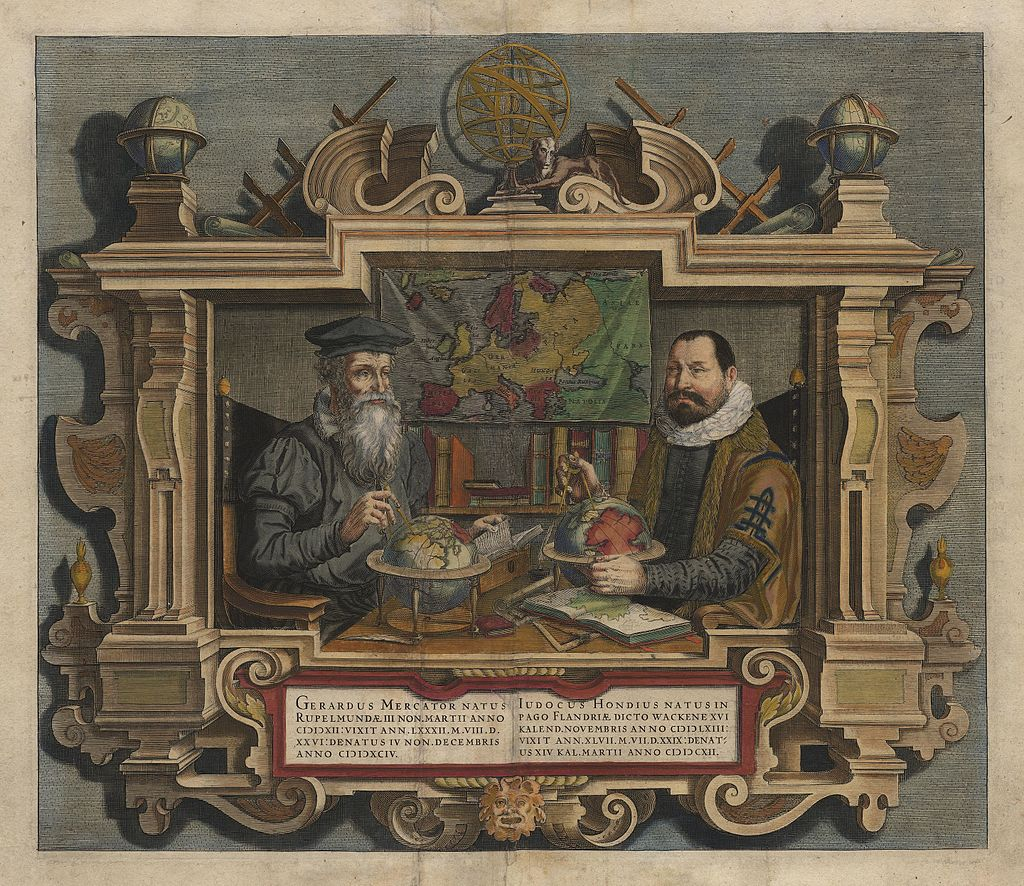
\includegraphics[width=1\linewidth]{../plots/Hondius_Portrait_of_map-makers}
				\caption{Portrait of map-makers, Gerard Mercator and Jodocus Hondius (Jodocus Hondius) source: \url{https://commons.wikimedia.org/wiki/File:Hondius_Portrait_of_map-makers.jpg}}
			\end{figure}
		\end{center}
	\end{column}
	\begin{column}{0.4\linewidth}
		\begin{center}
			\begin{itemize}
				\item<2-> Topography is a description of a landscape
				\item<3-> Topics (from the Greek \texttau\textomikron\textpi\textomikron\textvarsigma, place) can describe the features of a body of text
			\end{itemize}
		\end{center}
	\end{column}
\end{columns}
\end{frame}


\begin{frame}{Context}

\begin{columns}
	\begin{column}{0.5\linewidth}
		\begin{center}
			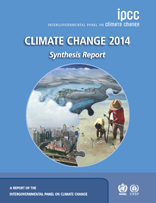
\includegraphics[width=0.6\linewidth]{syrcover.png}
		\end{center}
	\end{column}
	\begin{column}{0.5\linewidth}
		\begin{center}
			\begin{itemize}
				\item To contribute evidence-based policy-making on climate change, the IPCC aims to \textit{comprehensively} assess scientific literature on climate change 
				\item These assessments should be aim to balance legitimacy, credibility and relevance \citep{Cash2001}
			\end{itemize}
		\end{center}
	\end{column}
\end{columns}

\end{frame}


\begin{frame}{Motivation - Big Literature}

\begin{columns}
	\begin{column}{0.5\linewidth}
		\begin{figure}
			\includegraphics<1>[width=1\linewidth]{../plots/volume_variety_AR0}
			\includegraphics<2>[width=1\linewidth]{../plots/volume_variety_AR1}
			\includegraphics<3>[width=1\linewidth]{../plots/volume_variety_bible_AR1}
			\includegraphics<4>[width=1\linewidth]{../plots/volume_variety_bible_AR2}
			\includegraphics<5>[width=1\linewidth]{../plots/volume_variety_bible_AR3}
			\includegraphics<6>[width=1\linewidth]{../plots/volume_variety_bible_AR4}
			\includegraphics<7>[width=1\linewidth]{../plots/volume_variety_bible_AR5}
			\includegraphics<8->[width=1\linewidth]{../plots/volume_variety_bible_AR6}
		\end{figure}
	\end{column}
	\begin{column}{0.5\linewidth}
		\begin{center}
			\only<1>{\framebox[1.1\width]{A matrix of documents x words } \par}
			\only<2>{\framebox[1.1\width]{AR1: 1,848 documents x 3,528 words } \par}
			\only<3>{\begin{framed}
					The Luther Bible: 1,189 documents (chapters) x 11,973 words
			\end{framed}}
			%\only<3>{\framebox[1.1\width]{The Luther Bible: \par 1,189 documents (chapters) x 11,973 words } \par}
			\only<4>{\framebox[1.1\width]{AR2: 6,941 documents x 15,781 words } \par}
			\only<5>{\framebox[1.1\width]{AR3: 18,728 documents x 27,730 words } \par}
			\only<6>{\framebox[1.1\width]{AR4: 44,000 documents x 45,388 words } \par}
			\only<7>{\framebox[1.1\width]{AR5: 108,277 documents x 75,553 words } \par}
			\only<8->{\framebox[1.1\width]{AR6: 128,357 documents x 86,149 words } \par}
		\end{center}
		\only<9->{		
			\begin{center}
				\begin{itemize}
					\item Comprehensive, credible and relevant assessments become
					more challenging as the literature grows \citep{Minx2017l}
				\end{itemize}
				\begin{remark}[]
					To understand, and to aid, scientific assessments of climate change, we need to machine read the literature
				\end{remark}
			\end{center}
		}
	\end{column}
\end{columns}

\end{frame}



\begin{frame}{Approach - Words, words, words}

\begin{columns}
\begin{column}{0.5\linewidth}
	\begin{center}
		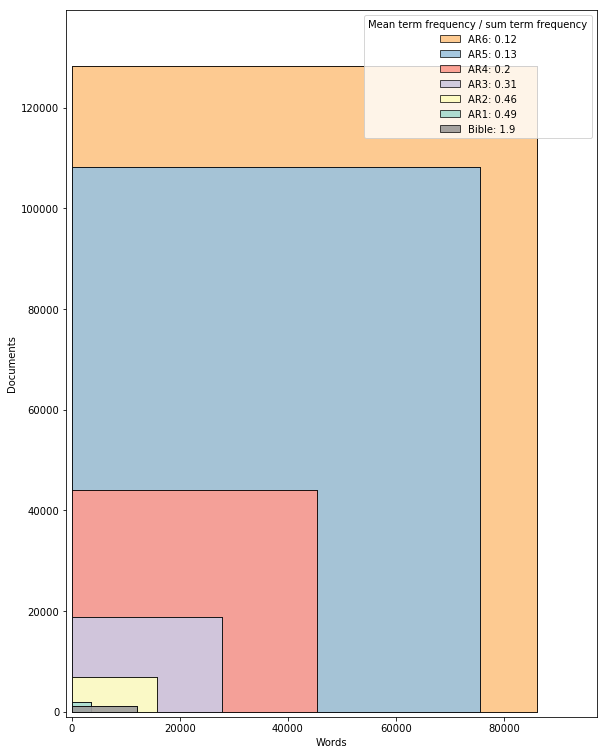
\includegraphics[width=\linewidth]{../plots/volume_variety_bible_AR6}
	\end{center}
\end{column}
\begin{column}{0.5\linewidth}
	\textbf{Topic Modelling}
	\begin{center}
		\begin{itemize}
			\item Topic modelling is a way of reducing the dimensionality of a corpus of documents
			\item A large matrix of documents x words is factorised by
			a matrix of topics x words and a matrix of topics x documents
			\citep{Lee1999}
			\item Topics describe the latent structure of the document corpus (What is the matter?)
			
		\end{itemize}
	\end{center}
\end{column}
\end{columns}

\end{frame}

\begin{frame}{Approach - Words, words, words}

\begin{figure}

\only<1>{\(V_{i\mu} \) is a term frequency-inverse document frequency matrix of \textit{stemmed} terms} 
\only<2>{\[V_{i\mu} \approx (WH)_{i\mu} = \sum_{a=1}^{r}W_{ia}H_{a\mu} \]} %\(V\) is approximated by the product of \(W\) and \(H\)}

\includegraphics<1>[width=\linewidth]{../plots/VWH_blank.png}
\includegraphics<2>[width=\linewidth]{../plots/VWH}

\only<1>{\caption{A topic model of 3495 documents on climate change from the year 2000}}

\only<2>{\caption{A topic model of 3495 documents on climate change from the year 2000}}

\end{figure}

\end{frame}


%%%%%%%%%%%%%%%%%%%%%%%%

\begin{frame}{Research Questions}
\begin{columns}
\begin{column}<1->{0.5\linewidth}
\begin{framed}
What is the thematic structure of the literature on climate change, and how has this changed over the five assessment periods of the IPCC
\end{framed}
\end{column}
\begin{column}<2->{0.5\linewidth}
\begin{framed}
What can this modelled thematic structure tell us about the relationship between the IPCC and scientific literature on climate change? How do the maps relate to the mapped?
\end{framed}
\end{column}
\end{columns}

\only<3->{
\textbf{Steps}
\begin{enumerate}
\item<4-> Download document metadata from Web of Science (WoS)
\item<5-> Match documents to reference lists from IPCC reports
\item<6-> Topic model stemmed document abstracts
\end{enumerate}
}
\end{frame}

%%

\begin{frame}{Data - Query}
\begin{columns}
\begin{column}{0.65\linewidth}
\tiny
(SO=(Climate Alert OR Climate Dynamics OR Climate Policy OR Climatic Change OR Global and Planetary Change OR Global Change Biology OR International Journal of Greenhouse Gas Control OR Mitigation and Adaptation Strategies for Global Change) OR TS=(((CO2 OR "carbon dioxide" OR methane OR CH4 OR "carbon cycle" OR "carbon cycles" OR "carbon cycling" OR "carbon budget*" OR "carbon flux*" OR "carbon mitigation") AND (climat*)) OR (("carbon cycle" OR "carbon cycles" OR "carbon cycling" OR "carbon budget*" OR "carbon flux*" OR "carbon mitigation") AND (atmospher*))) OR TS=("carbon emission*" OR "sequestration of carbon" OR "sequester* carbon" OR "sequestration of CO2" OR "sequester* CO2" OR "carbon tax*" OR "CO2 abatement" OR "CO2 capture" OR "CO2 storage" OR "CO2 sequester*" OR "CO2 sequestration" OR "CO2 sink*" OR "anthropogenic carbon" OR "captur* of carbon dioxide" OR "captur* of CO2" OR "climat* variability" OR "climat* dynamic*" OR "chang* in climat*" OR "climat* proxies" OR "climat* proxy" OR "climat* sensitivity" OR "climat* shift*" OR "coupled ocean-climat*" OR "early climat*" OR "future climat*" OR "past climat*" OR "shift* climat*" OR "shift in climat*") OR TS=("atmospheric carbon dioxide" OR "atmospheric CH4" OR "atmospheric CO2" OR "atmospheric methane" OR "atmospheric N2O" OR "atmospheric nitrous oxide" OR "carbon dioxide emission*" OR "carbon sink*" OR "CH4 emission*" OR "climat* policies" OR "climat* policy" OR "CO2 emission*" OR dendroclimatolog* OR ("emission* of carbon dioxide" NOT nanotube*) OR "emission* of CH4" OR "emission* of CO2" OR "emission* of methane" OR "emission* of N2O" OR "emission* of nitrous oxide" OR "historical climat*" OR IPCC OR "methane emission*" OR "N2O emission*" OR "nitrous oxide emission*") OR TS=("climat* change*" OR "global warming" OR "greenhouse effect" OR "greenhouse gas*" OR "Kyoto Protocol" OR "warming climat*" OR "cap and trade" OR "carbon capture" OR "carbon footprint*" OR "carbon neutral" OR "carbon offset" OR "carbon sequestration" OR "carbon storage" OR "carbon trad*" OR "changing climat*" OR "climat* warming")) NOT PY=2018

\normalsize
\begin{itemize}
\item \citep{Haunschild2016}
\item 309,697 documents
\end{itemize}
\end{column}
\begin{column}{0.35\linewidth}
\textbf{Caveats}
\begin{itemize}
\item Not perfect query (Expressio Unius Est Exclusio Alterius )
\item WoS not all peer-reviewed literature
\item Missing grey literature
\item Missing relevant literature not directly about climate change
\end{itemize}
\end{column}
\end{columns}
\end{frame}

\begin{frame}{Data - IPCC References}
\textbf{Matching process}

\medskip

For each Reference:
\begin{itemize}
\item Check for case-insensitive title matches
\item Calculate the Jaccard similarity score for two word shingles every database document containing the first word and from the same year. Match if the Jaccard score is above 0.45
\end{itemize}
\end{frame}


\begin{frame}{Data - IPCC References}
%\begin{columns}
%\begin{column}{0.5\linewidth}
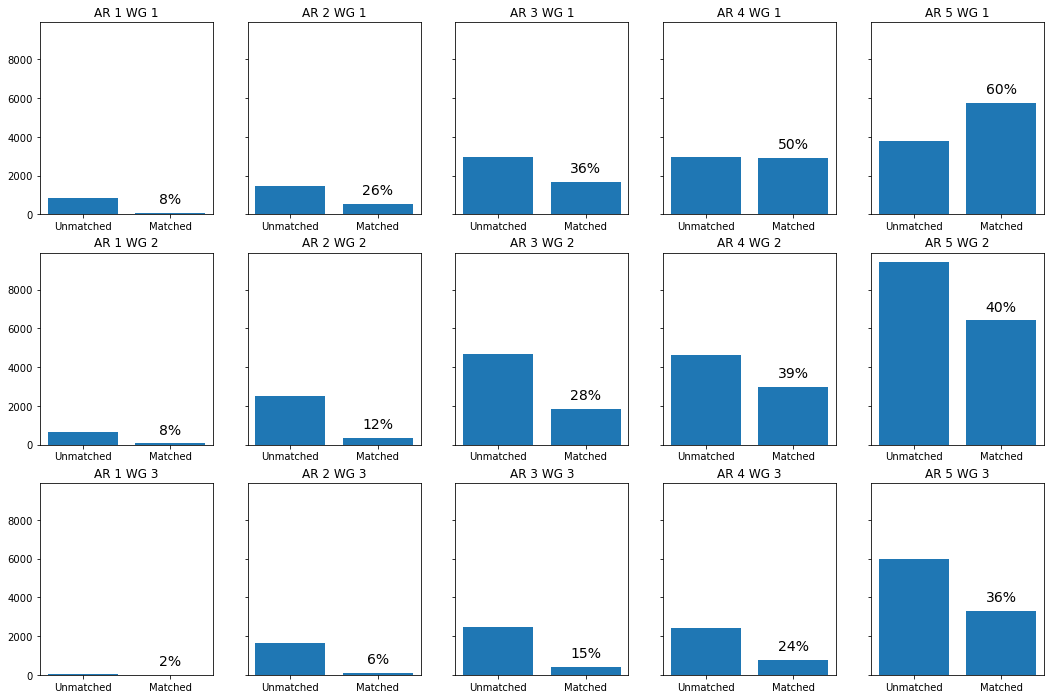
\includegraphics[width=\linewidth]{../plots/ipcc_matches}
%\end{column}
%\end{columns}
\end{frame}

\begin{frame}{Data - Unmatched IPCC References}

37\% of IPCC References could be matched to the database of climate-relevant documents

\medskip

\textbf{Reasons for not matching}
\begin{enumerate}
\item<2->Reference is not in WoS (not peer-reviewed, in minor journal)
\item<3->Reference is not directly about climate change
\item<4->Reference has been incorrectly parsed
\end{enumerate}

\medskip

\only<5->{\textbf{Observations}}
\begin{itemize}
\item<5-> The size of the literature appears to be \textit{much} bigger than our estimate
\item<6-> WG3 refers to more literature not directly about climate change, or not in peer-reviewed publications, than WG2, which refers to more than WG1
\end{itemize}

\end{frame}

\begin{frame}{Data - Unmatched IPCC References}
\tiny
\begin{tabular}{l l p{4.5cm} p{2.5cm} r}
\toprule
 AR &  WG &                                                                                                                                                                           text &                                                            authors &  year \\
\midrule
 3 &  1 &  The IIASA Database for Mean Monthly   Values of Temperature, Precipitation and Cloudiness on a Global Terrestrial   Grid. IIASA Report RR-91-18, Laxenburg, 63 pp. &  Leemans, R. and W. Cramer &  1991 \\
 2 &  2 &  Rischi connessi con la dinámica glaciale nelle Alpi ItaUane. Geografía Física e Dinámica Quatemaría, 15, 85-99.  &  Dutto, F. and G. Mortara &  1992 \\
 3 &  1 &  Specification   of eddy transfer coefficients in coarse-resolution ocean circulation models.   J. Phys. Oceanogr., 27, 381-402. &  Visbeck, M., J. Marshall, T. Haine and M. Spall &  1997 \\
 3 &  2 &  A koala (Phascolartos   cinereus Goldfuss) population crash during drought and heatwave conditions in   south-western Queensland. Australian Journal of Ecology, 13, 451-461. &  Gordon, G., A.S. Brown, and T. Pulsford &  1988 \\
 4 &  2 &  Climate change and land resources of Russia. &  Isaev, A., V. Stolbovoi, V. Kotlyakov, S. Nilsson and I. McCallum &  2004 \\
 4 &  3 &  Generation technology choices: near and long term. US DOE/EPRI Annual Energy Outlook Conference, Washington D.C., www.eia.doe.gov/oiaf/archive/aeo04/conf/pdf/gehl.pdf  &  Gehl, S &  2004 \\
 4 &  3 &  Climate Change and the European Countryside: Impacts on Land Management and Response Strategies &  Viner, D., M. Sayer, M. Uyarra, and N. Hodgson &  2006 \\
 5 &  2 &  Adaptation to climate change in the context ofsustainable development and equity &  Smit, B. and O. Pilifosova &  2001 \\
 5 &  3 &  Copenhagen City of Cyclists: Bicycle Account 2010. City of Copenha-gen, The Technical and Environmental Administration. Available at: http: / / www. cycling-embassy &  COP &  2010 \\
 5 &  3 &  Uncertainty analysis of the IEA / ORAU CO2 emissions model. The Energy Journal 8, 1 – 29 &  Reilly J M, J A Edmonds, R H Gardner, and A L Brenkert &  1987 \\
\bottomrule
\end{tabular}

\end{frame}

\begin{frame}{Methodology - Dynamic Topic Modelling}

The topic models above assume that the topics, and the words that make them up, are stable over time. Two approaches to better model dynamic topics:

\begin{itemize}
\item<2->Dynamic Topic Modelling (DTM) \citep{Blei2006} assume that a constant number of topics exists over all topic models, but allows the words in the topics to evolve from one time period to another
\item<3->Dynamic Non-negative Matrix Factorisation \citep{Greene2016} has varying numbers of topics in each window and allows for topics to emerge and/or disappear.
\end{itemize}

\onslide<4->{Where the size and variety of the literature we want to model has increased exponentially, we need an approach that allows for the emergence of new topics.}

\end{frame}

%%%%%%%%%%%%%%%%%%%%%%%
%% D-NMF


\begin{frame}[t]{Dynamic NMF}


\only<1->{
\includegraphics[]{../plots/sustainability/VWH_1991}}
\only<2->{
\includegraphics[]{../plots/sustainability/VWH_1992}}

\only<3->{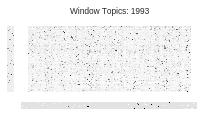
\includegraphics[]{../plots/sustainability/VWH_1993}}

\end{frame}

\begin{frame}[t]{Dynamic NMF}

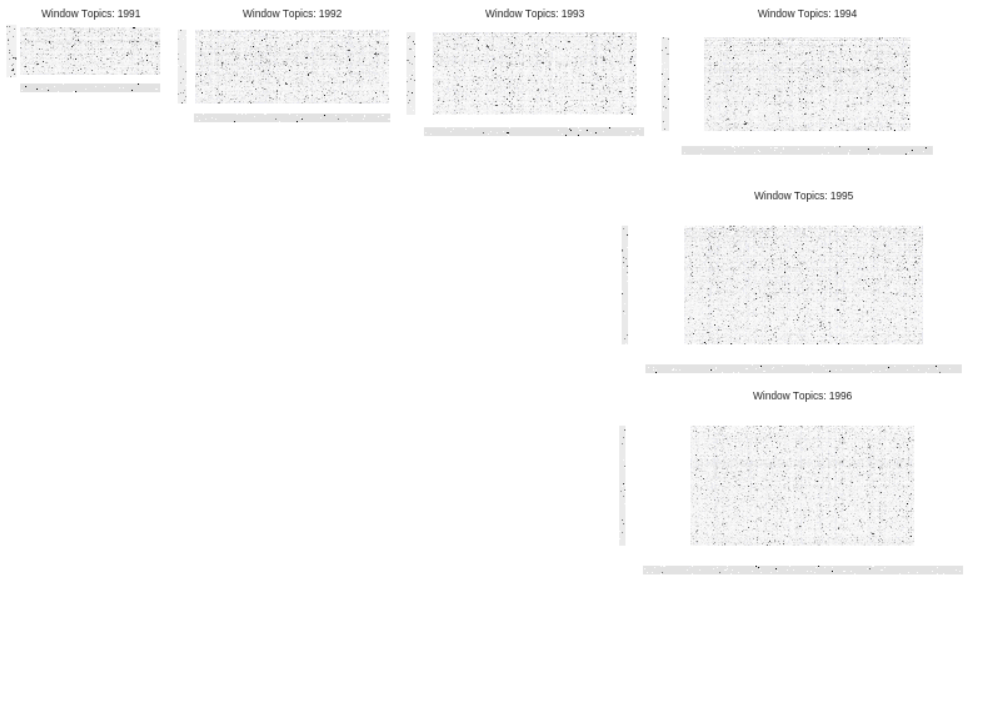
\includegraphics[width=\linewidth]{../plots/sustainability/conceptual_windows_only}

\end{frame}

\begin{frame}[t]{Dynamic NMF}

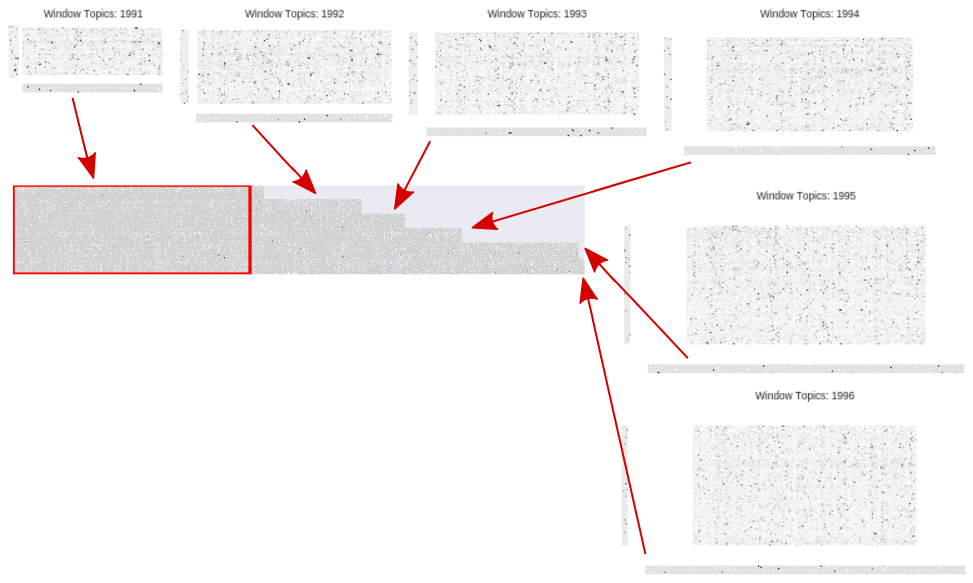
\includegraphics[width=\linewidth]{../plots/sustainability/conceptual_annotated_1}

\end{frame}

\begin{frame}[t]{Dynamic NMF}

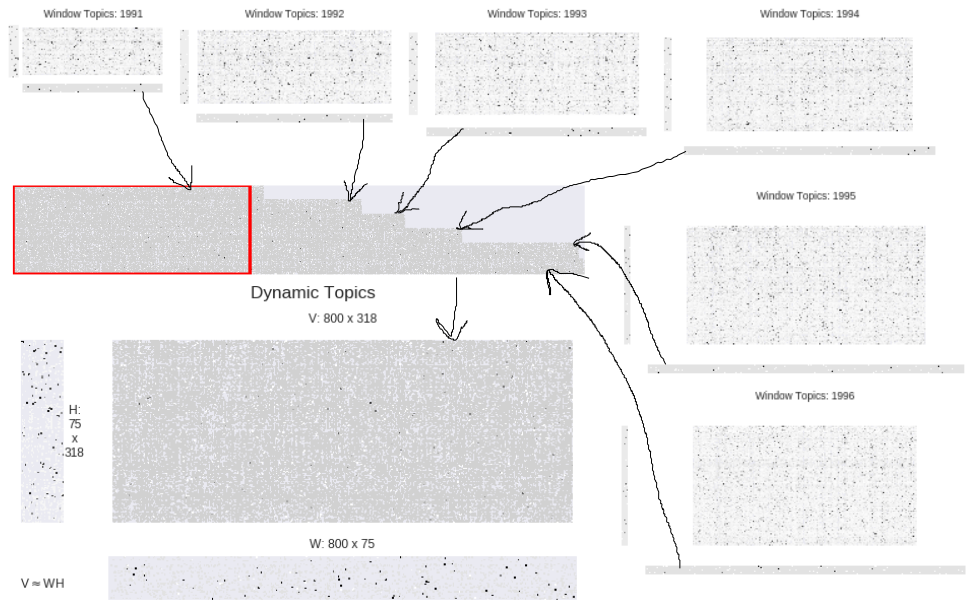
\includegraphics[width=\linewidth]{../plots/sustainability/conceptual_annotated_2}

\end{frame}



%%%%%%%%%%%%%%%%%%%%%%%%%%%%%%%%%%%
% results

\begin{frame}{Results}

\begin{columns}
	\begin{column}{0.75\linewidth}
		\begin{figure}	
			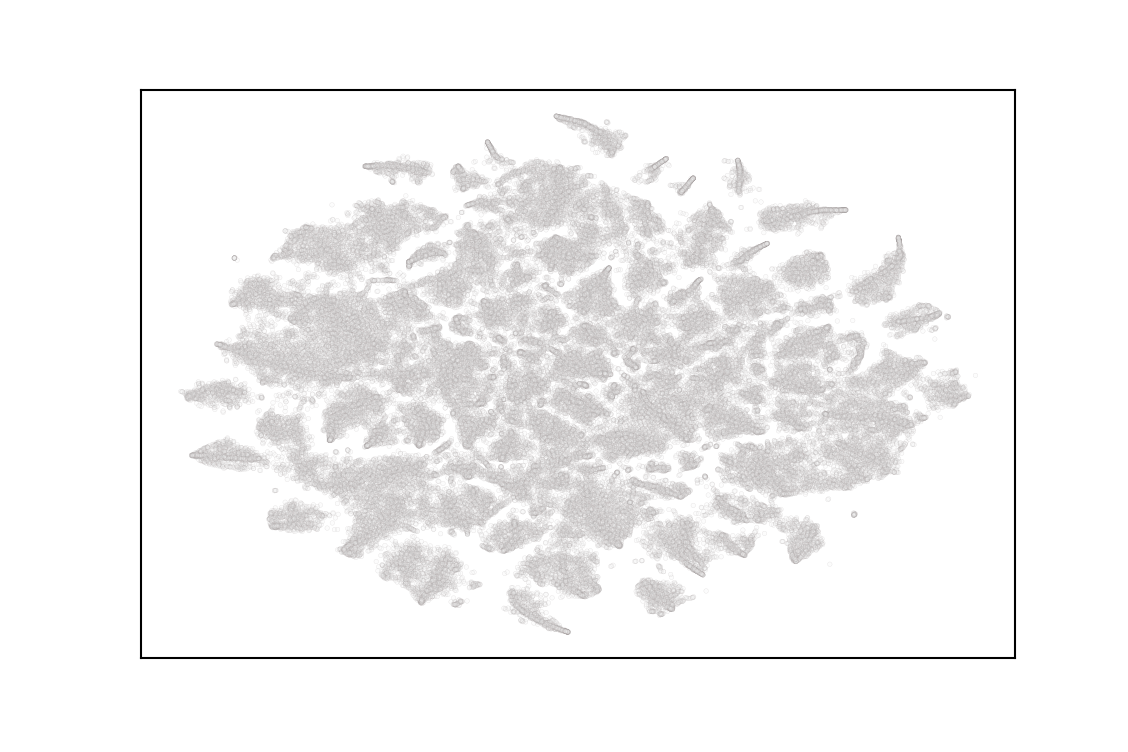
\includegraphics[width=\linewidth]{../tsne_results/plots/run_662_s_100000_p30_blank}
			\caption{A topographical representation of 100,000 documents on climate change}
		\end{figure}
	\end{column}
	\begin{column}{0.25\linewidth}
		\textbf{Outline}	
		\begin{center}
			\begin{itemize}
				\item<2-> Topography
				\item<4-> Development
				\item<5-> Representation in IPCC reports
				%\item<6-> AR6 outlook
			\end{itemize}
		\end{center}
	\end{column}
\end{columns}

\end{frame}

\begin{frame}{Results - Topography}

\begin{columns}
	\begin{column}{0.7\linewidth}
		\begin{figure}	
			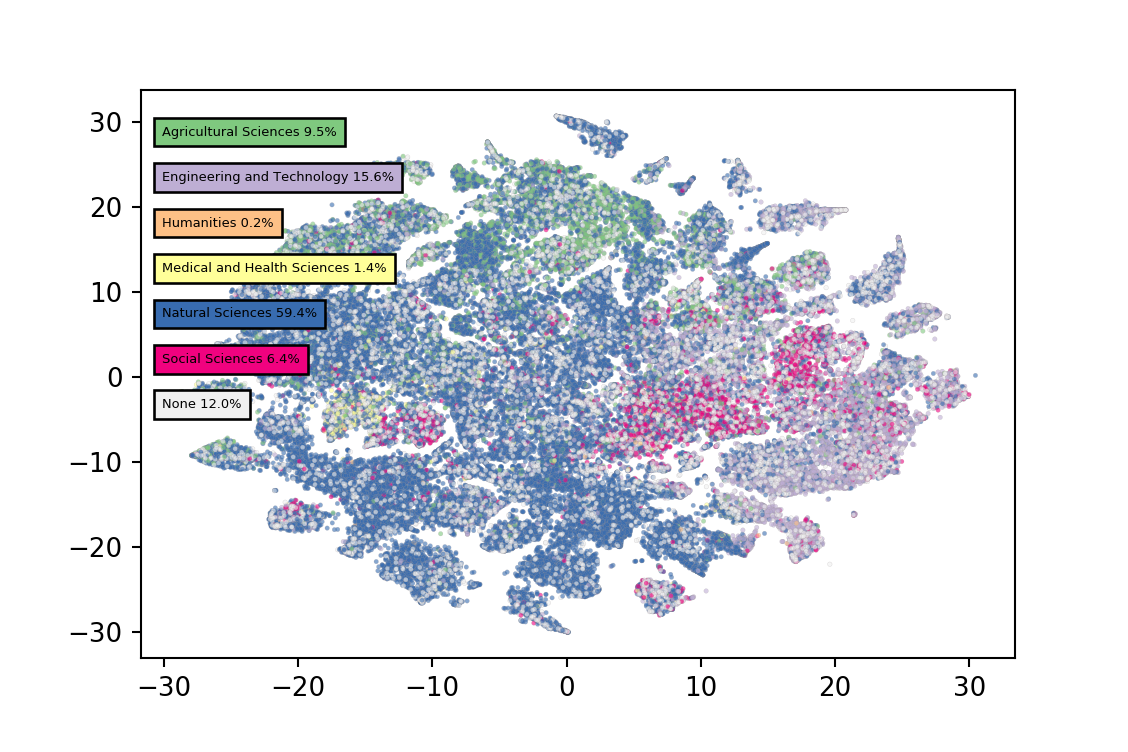
\includegraphics[width=\linewidth]{../tsne_results/plots/run_662_s_100000_p30_oecds}
			\caption{A topographical representation of 100,000 documents on climate change. Document positions are dictated by topic scores, reduced to two dimensions through t-SNE}
		\end{figure}
	\end{column}
	\begin{column}{0.3\linewidth}	
		\begin{center}
			\begin{itemize}
				\item<2-> t-distributed stochastic neighbour embedding (t-SNE) \citep{vandermaaten2008} places nodes with similar topic scores close together
				\item<3-> This \textit{projects} the 100-dimensional topic scores onto a conventional 2-dimensional topographical map
				\item<4-> Topics cut across journal disciplinary categories, but the disciplinary structure remains visible
			\end{itemize}
		\end{center}
	\end{column}
\end{columns}

\end{frame}

\begin{frame}{Results - Topography}

\begin{columns}
	\begin{column}{0.7\linewidth}
		\begin{figure}	
			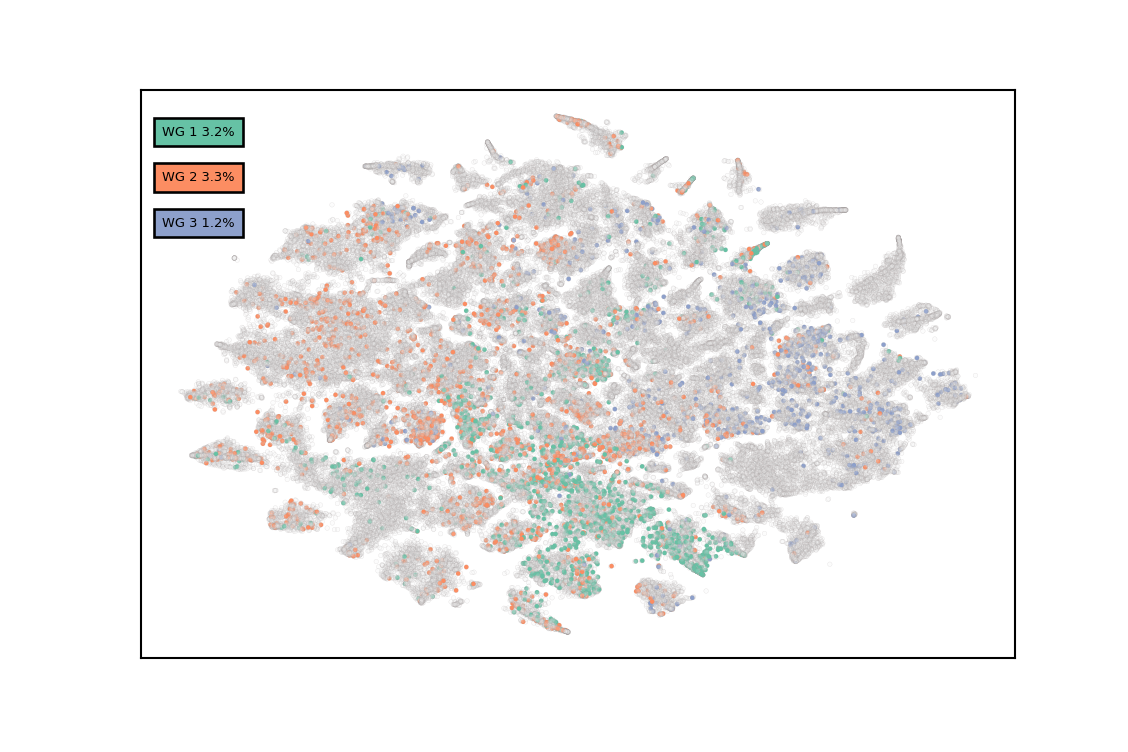
\includegraphics[width=\linewidth]{../tsne_results/plots/run_662_s_100000_p30_wgs}
			\caption{A topographical representation of 100,000 documents on climate change. Document positions are dictated by topic scores, reduced to two dimensions through t-SNE, nodes are coloured by references by IPCC reports}
		\end{figure}
	\end{column}
	\begin{column}{0.3\linewidth}	
		\begin{center}
			\begin{itemize}
				\item<1-> The disciplinary structure fits with the pattern of citations by IPCC reports
				\item<2-> Citations by IPCC reports are densest in WGI/Natural science topical areas.
			\end{itemize}
		\end{center}
	\end{column}
\end{columns}

\end{frame}

\begin{frame}{Results - IPCC Representation}

\begin{columns}
	\begin{column}{0.65\linewidth}
		\begin{figure}	
			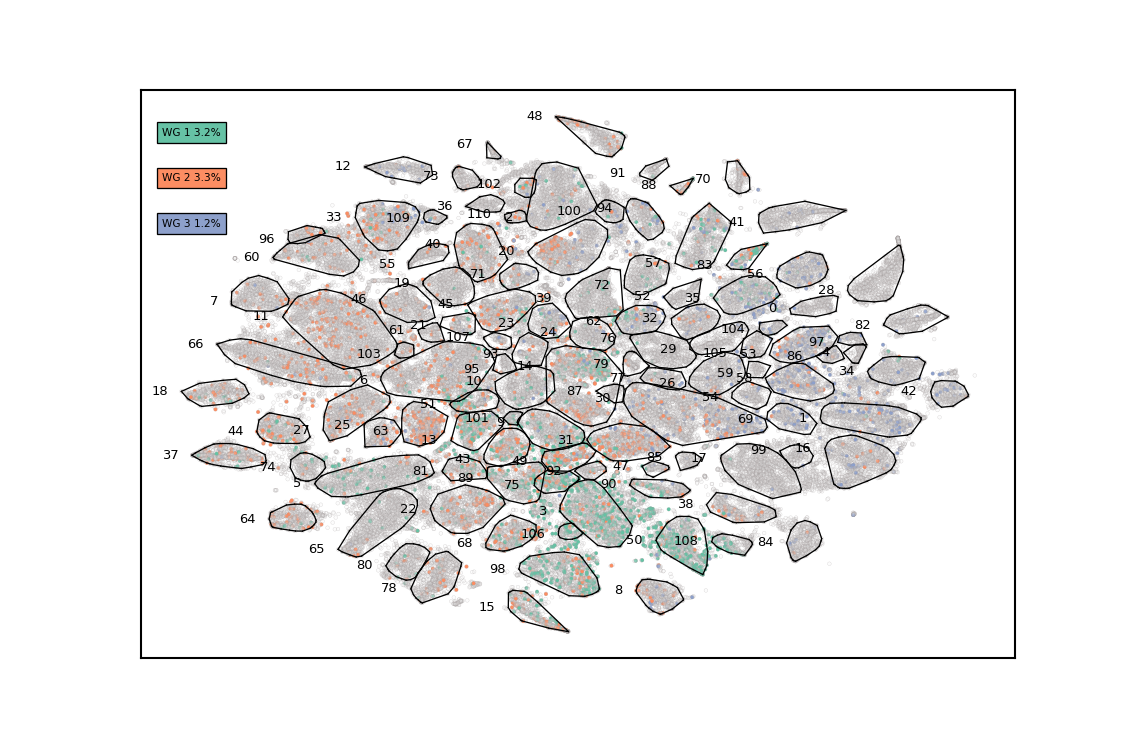
\includegraphics[width=\linewidth]{../tsne_results/plots/run_662_s_100000_p30_clusters_wgs.png}
			\caption{Clusters of documents}
		\end{figure}
	\end{column}
	\begin{column}{0.35\linewidth}	
		\begin{center}
			\begin{itemize}
				\item<1-> We can identify clusters of documents, each of which are dominated by topics or clusters of topics
				\item<2-> 58 is a mixture of economics, policies and taxes, and emissions reductions
				\item<3-> 41 is on CO2 storage
				\item<4-> 11 is on species and habitats
				\item<5-> 33 is on forests
			\end{itemize}
		\end{center}
	\end{column}
\end{columns}

\end{frame}

\begin{frame}{Results - Topography}

	\begin{figure}	
		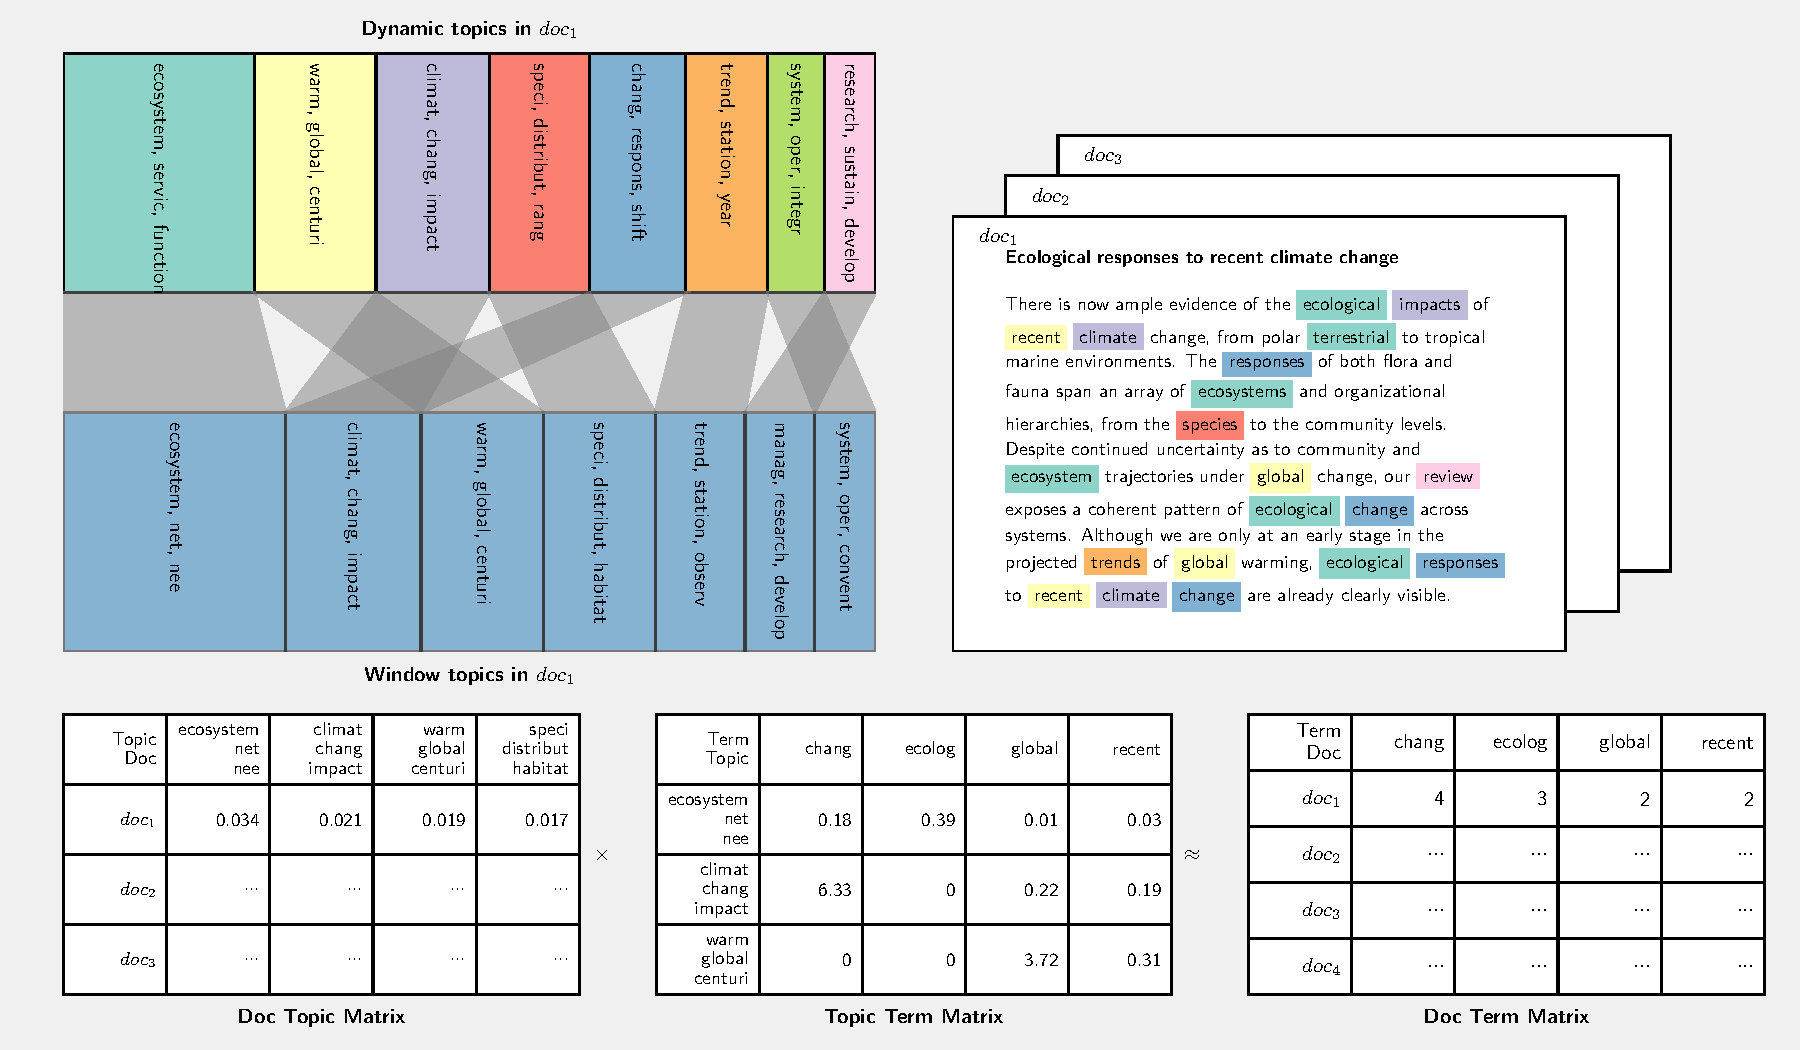
\includegraphics[width=\linewidth]{../plots/single_doc_3_536594.pdf}
		\caption{How topics describe documents}
	\end{figure}

\end{frame}

\begin{frame}{Results - Development}

\begin{figure}	
	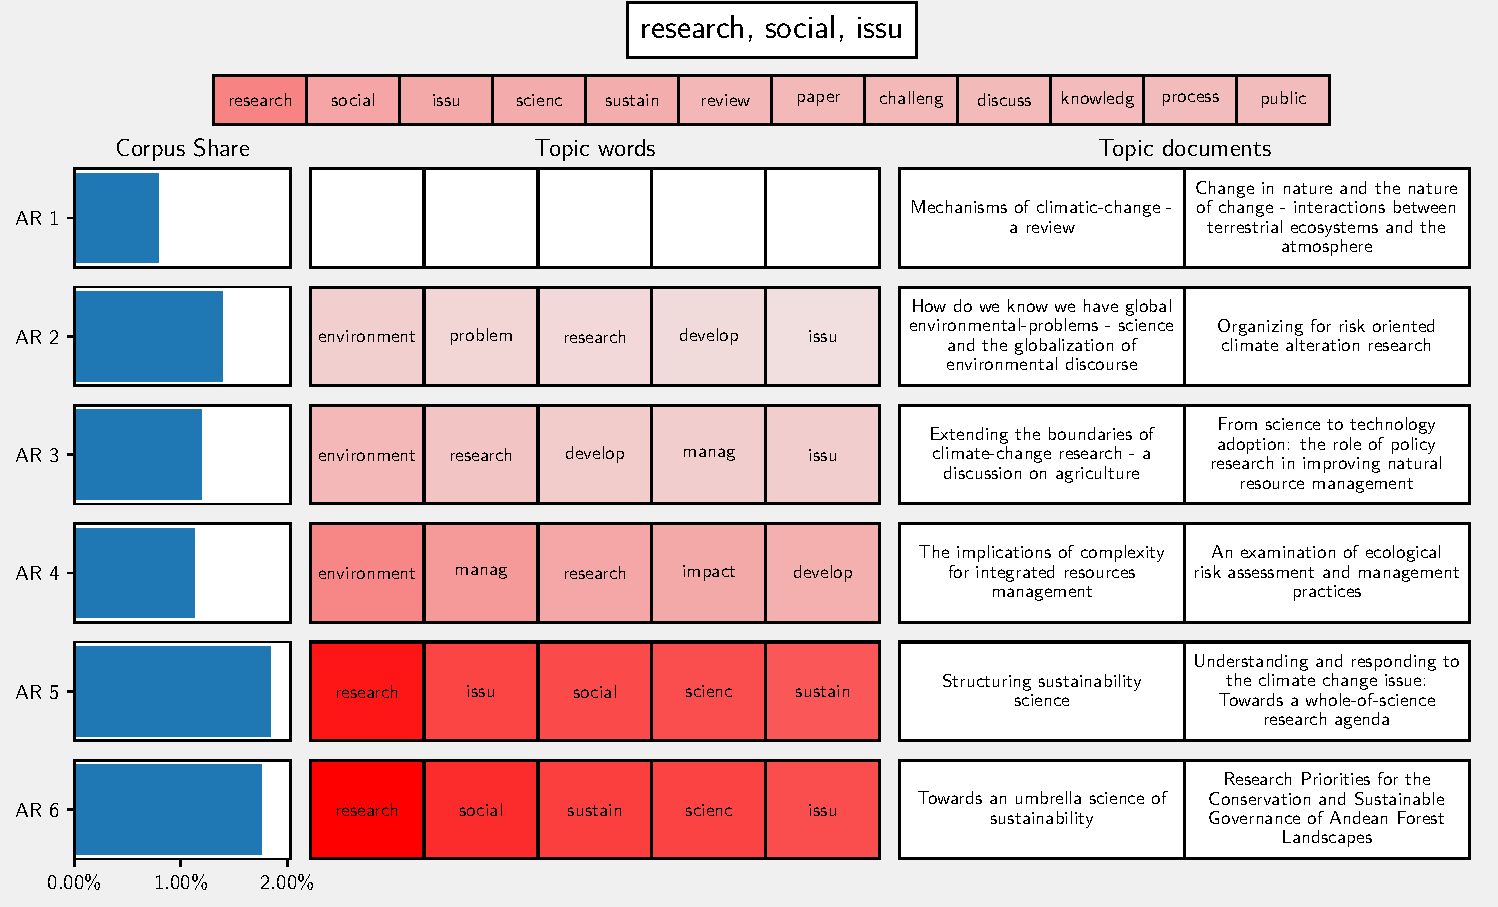
\includegraphics[width=\linewidth]{../plots/single_topic_3_11046.pdf}
	\caption{The evolution of topics}
\end{figure}

\end{frame}

\begin{frame}{Results - Development}

\begin{figure}	
	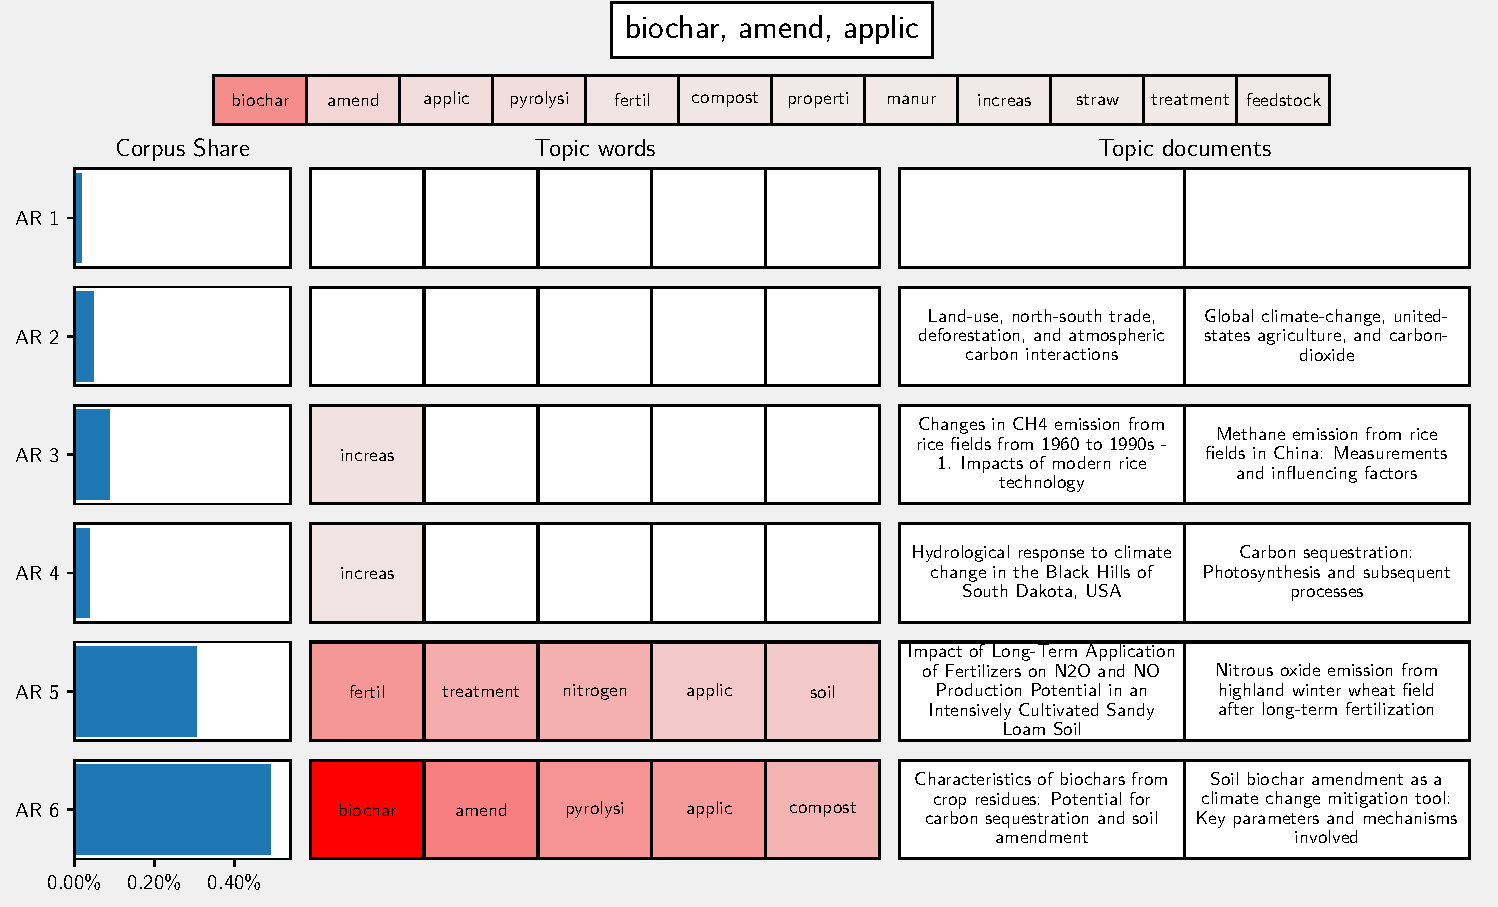
\includegraphics[width=\linewidth]{../plots/single_topic_3_11020.pdf}
	\caption{The emergence of new topics}
\end{figure}

\end{frame}

\begin{frame}{Results - Development}

\begin{figure}	
	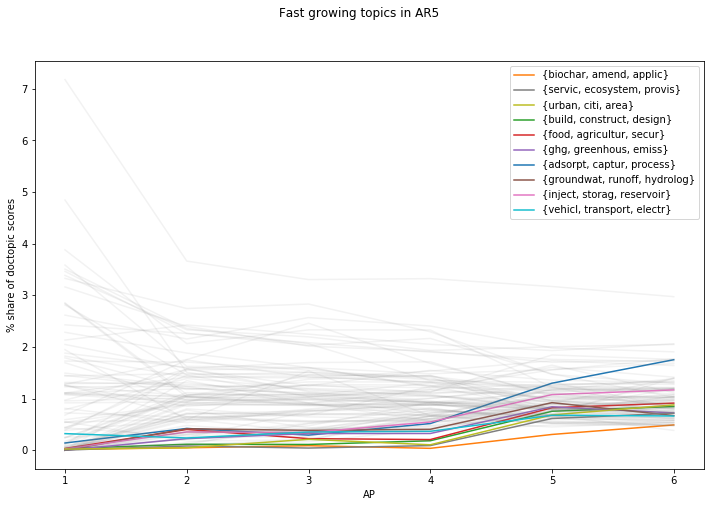
\includegraphics[width=\linewidth]{../plots/ar5_growth_665.png}
	\caption{The emergence of new topics}
\end{figure}

\end{frame}

\begin{frame}{Results - IPCC representation}

\begin{itemize}
	\item<1-> How can we get a sense of which topics are better covered in IPCC reports?
	\item<2-> We get a measure of proportionality between two distributions by dividing each topic's share in the IPCC sample by its share in the whole corpus
	\item<3-> This and other measures come from literature on the proportionality of electoral systems \citep[e.g][]{Karpov2008}
\end{itemize}


\end{frame}

\begin{frame}{Results - IPCC Representation}

\begin{columns}
	\begin{column}{0.65\linewidth}
		\begin{figure}	
			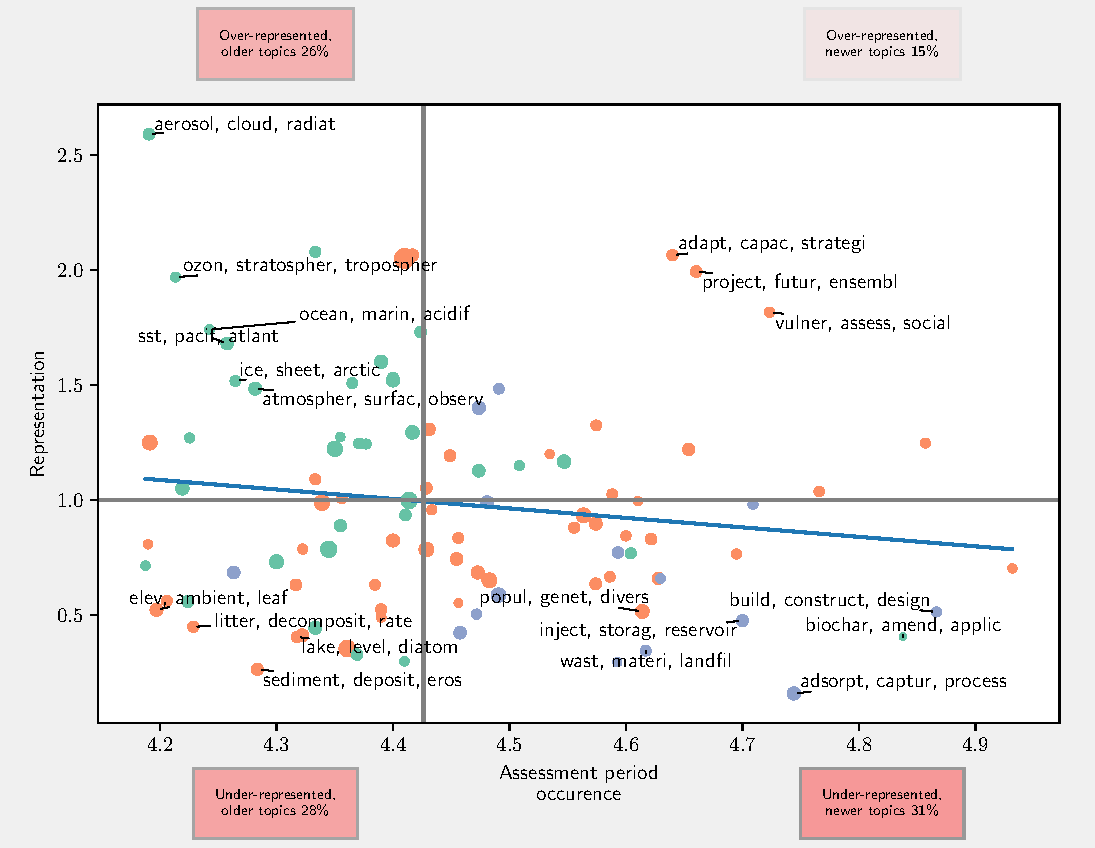
\includegraphics[width=\linewidth]{../plots/ipcc_representation/ipcc_rep_new665_all.pdf}
			\caption{New and old, better and less well represented topics}
		\end{figure}
	\end{column}
	\begin{column}{0.35\linewidth}	
		\begin{center}
			\begin{itemize}
				\item<1-> Topics on the scientific basis of climate change are well represented in IPCC reports and have been around longer than average
				\item<2->Topics on impacts have seen lots of recent growth, and are well represented in IPCC reports
				\item<3->Topics on ``solutions'', or on new technologies or contexts for mitigation have seen lots of recent growth, but are under-represented in IPCC reports
			\end{itemize}
		\end{center}
	\end{column}
\end{columns}

\end{frame}

\begin{frame}{Robustness}

Most work focuses on the measuring the sensitivity of the reconstruction error to different framings and parameters of the model. What we are more interested in is checking if the key messages are sound.

\begin{columns}<2->
	\begin{column}<3->{0.33\linewidth}
		\begin{figure}
			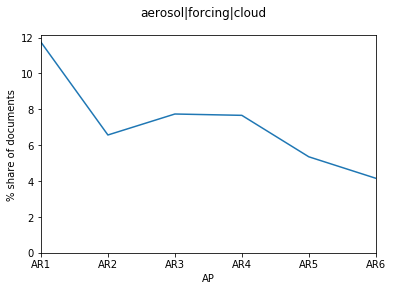
\includegraphics[width=\linewidth]{../plots/aero_share}
		\end{figure}
	\end{column}
	
	\begin{column}<4->{0.33\linewidth}
		\begin{figure}
			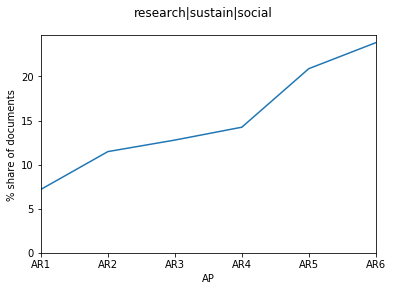
\includegraphics[width=\linewidth]{../plots/sus_share}
		\end{figure}
	\end{column}
	
\end{columns}
\begin{columns}
	
	\begin{column}<5->{0.33\linewidth}
		\begin{figure}
			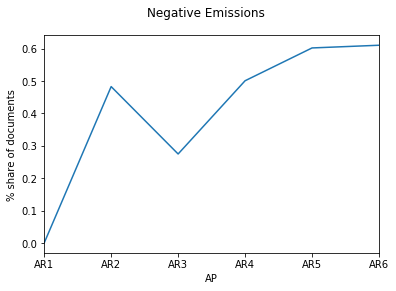
\includegraphics[width=\linewidth]{../plots/negative_emissions_share}
		\end{figure}
	\end{column}
	
	\begin{column}<6->{0.33\linewidth}
		\begin{figure}
			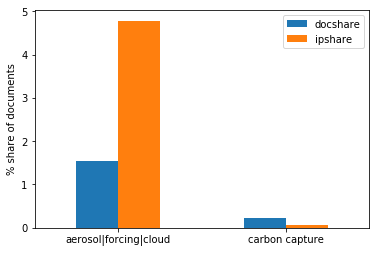
\includegraphics[width=\linewidth]{../plots/ipcc_rep_simple}
		\end{figure}
	\end{column}
\end{columns}

\end{frame}


\begin{frame}{Conclusions}


\begin{itemize}
	\item<1-> Endogenously discovered topics map and make substantive sense of an unmanageable dataset of climate-relevant literature
	\item<2-> Topic modelling discovers over-arching topics such as that on sustainability and research priorities, as well as specific, fast growing topics such those on negative emissions
	\item<3-> Some quantitative evidence is found to support policy makers' dissatisfaction with a lack of `solution orientation' in IPCC reports \citep{Kowarsch2017} 
\end{itemize}

\end{frame}

\begin{frame}{Discussion}


\begin{itemize}
\item<1-> A perfectly representative relationship between the literature and IPCC reports is not necessarily desirable
\item<2-> The IPCC are best placed to decide which aspects of the literature to emphasise
\item<3-> A topography of the literature helps to address issues of emphasis from a point of understanding, and to make decisions clear and transparent
\item<4-> More generally, maps like this present exciting opportunities to aid the process of literature selection, and to understand the science policy process
\end{itemize}

\end{frame}

\begin{frame}{A Topography of Climate Change Research}
\begin{columns}
	\begin{column}{0.5\linewidth}
		\begin{center}
			\begin{figure}
				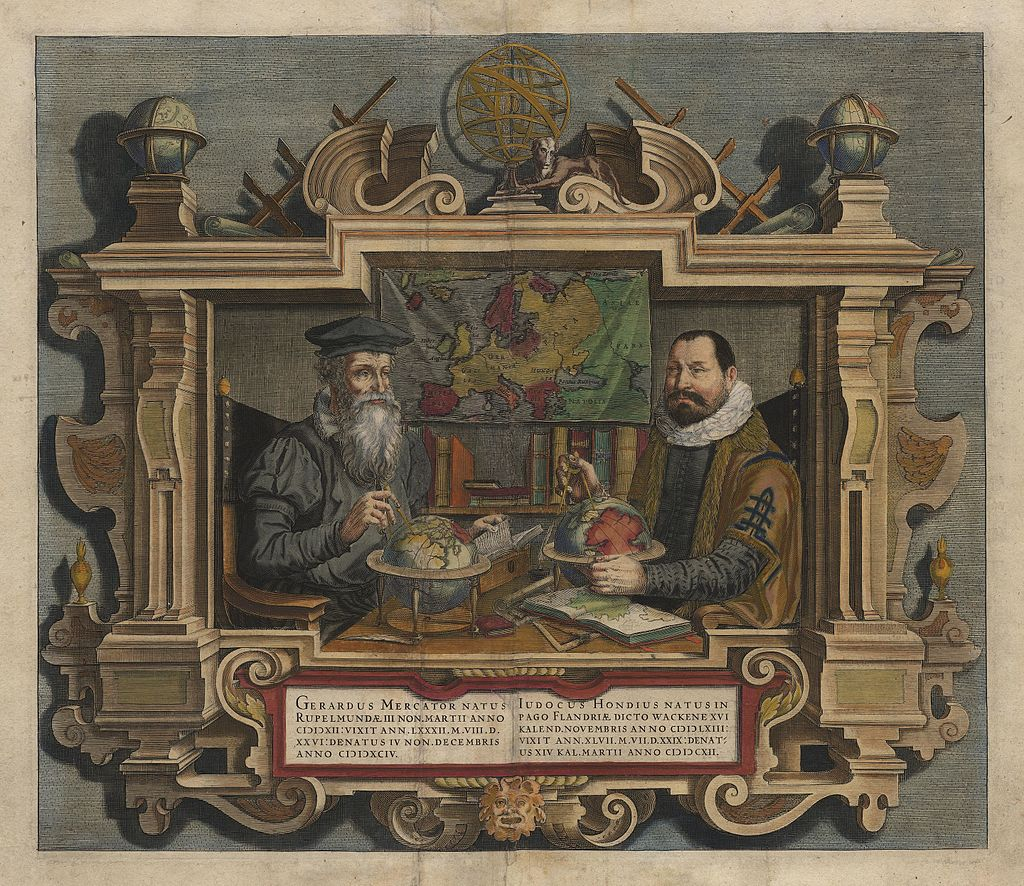
\includegraphics[width=1\linewidth]{../plots/Hondius_Portrait_of_map-makers}
				\caption{Portrait of map-makers, Gerard Mercator and Jodocus Hondius (Jodocus Hondius) source: \url{https://commons.wikimedia.org/wiki/File:Hondius_Portrait_of_map-makers.jpg}}
			\end{figure}
		\end{center}
	\end{column}
	\begin{column}{0.5\linewidth}
		\begin{center}
			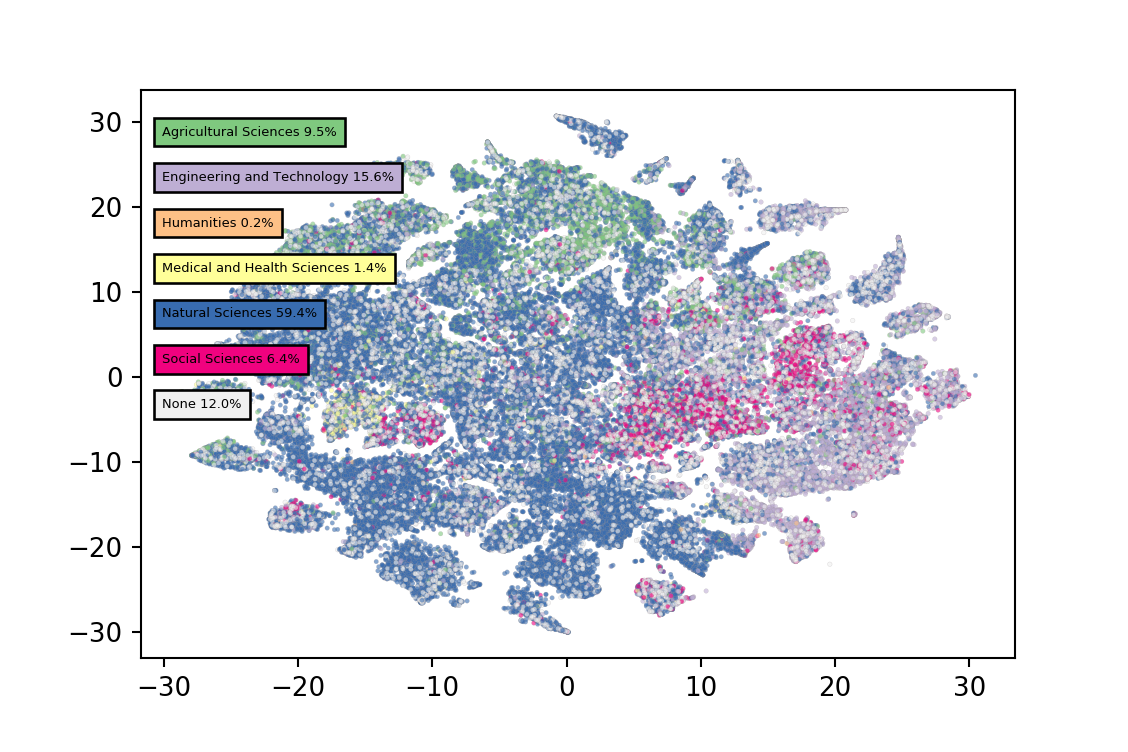
\includegraphics[width=\linewidth]{../tsne_results/plots/run_662_s_100000_p30_oecds}
		\end{center}
	\end{column}
\end{columns}
\end{frame}


%%%%%%%%%%%%%%%%%%%%%%%%%%%%%%
%% Bib

\begin{frame}{Bibliography}
\small
\bibliography{../Mendeley.bib}
\end{frame}

%%%%%%%%%%%%%%%%%%%%%%%%%%%%%%%%%%%
%% Extra slides

\appendix
\backupbegin

\begin{frame}{Robustness}

Most work focuses on the measuring the sensitivity of the reconstruction error to different framings and parameters of the model. What we are more interested in is checking if the key messages are sound.

\begin{columns}<2->
	\begin{column}<3->{0.33\linewidth}
		\begin{figure}
			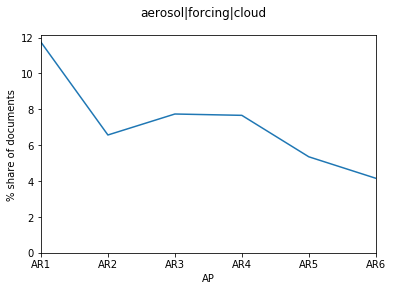
\includegraphics[width=\linewidth]{../plots/aero_share}
		\end{figure}
	\end{column}
	
	\begin{column}<4->{0.33\linewidth}
		\begin{figure}
			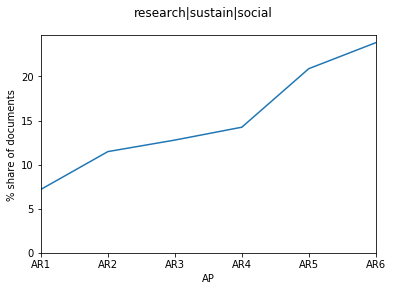
\includegraphics[width=\linewidth]{../plots/sus_share}
		\end{figure}
	\end{column}
	
\end{columns}
\begin{columns}
	
	\begin{column}<5->{0.33\linewidth}
		\begin{figure}
			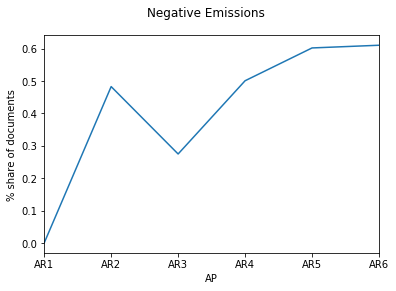
\includegraphics[width=\linewidth]{../plots/negative_emissions_share}
		\end{figure}
	\end{column}
	
	\begin{column}<6->{0.33\linewidth}
		\begin{figure}
			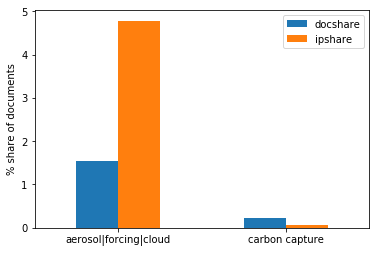
\includegraphics[width=\linewidth]{../plots/ipcc_rep_simple}
		\end{figure}
	\end{column}
\end{columns}

\end{frame}


\begin{frame}{Dynamic NMF - application to climate change}

\onslide<1->{
	\begin{itemize}
		\item Choosing the number of window topics is non-trivial. Data-driven approaches are limited (see below), and human selection is time consuming.
		\item To facilitate the description of trends over the assessment periods of the IPCC, and to minimize the number of modelling decisions, I consider each IPCC assessment period as a time window.
\end{itemize}}

\begin{columns}
	\onslide<2->{
		\begin{column}{0.5\linewidth}
			
			\begin{itemize}
				\item Starting from a logarithmic relationship between the number of documents and the ideal topic number, I compare 5 runs with varying numbers of topics for each window
			\end{itemize}
		\end{column}
		\begin{column}{0.5\linewidth}
			\begin{figure}
				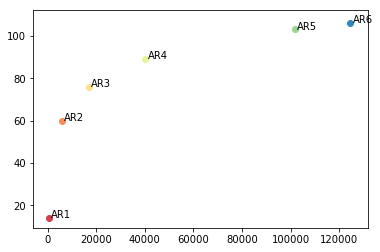
\includegraphics[width=\linewidth]{../plots/n_topics}	
			\end{figure}
		\end{column}
	}
\end{columns}

\end{frame}





\begin{frame}[t]{Dynamic NMF - number of topics}

\begin{columns}
\begin{column}{0.5\linewidth}
	\textbf{Human topic number criteria}
	\begin{itemize}
		\item Intelligibility
	\end{itemize}
	\textbf{Data-driven topic number criteria}
	\begin{itemize}
		\item Reconstruction accuracy
		\item Predictive capacity
	\end{itemize}
	\onslide<2->{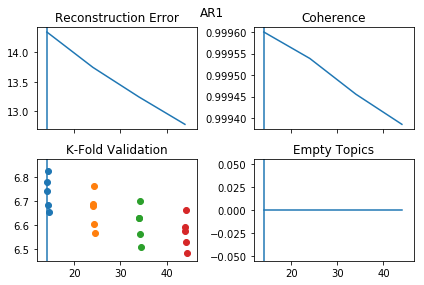
\includegraphics[width=0.8\linewidth]{../plots/topic_validations_AR1}}
\end{column}
\begin{column}<2->{0.5\linewidth}
	
	\begin{figure}
		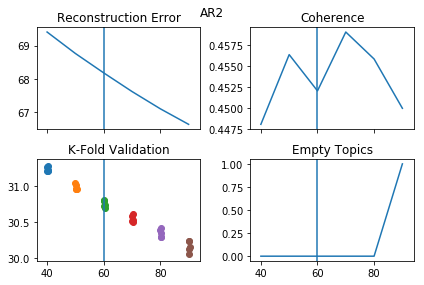
\includegraphics[width=0.8\linewidth]{../plots/topic_validations_AR2}
		
		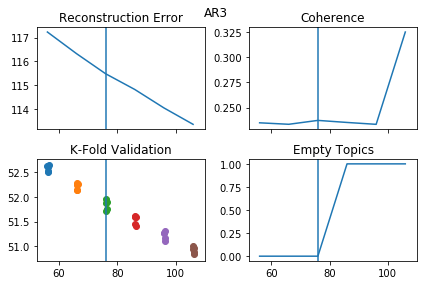
\includegraphics[width=0.8\linewidth]{../plots/topic_validations_AR3}
	\end{figure}
\end{column}
\end{columns}


\end{frame}

\backupend

\end{document}